\chapter{METHODOLOGY}
\section{System Design}

	The purpose of the helmet detection system is to track helmet use from CCTV footage on a college campus. Data preparation, model training, and counting implementation are the three primary phases of the system. The first step involves converting campus CCTV video footage into image frames, which are subsequently labelled with helmet and unhelmeted head information using Roboflow. A customised YOLOv8 object detection model that is tuned for real-time performance is trained using the annotated dataset. After training, the model is incorporated into a real-time system that recognises and categorises heads and helmets by processing incoming video frames. In order to provide real-time statistics that facilitate safety compliance monitoring, a counting mechanism is integrated to monitor the quantity of helmets and heads seen within a designated area of interest.
	

\begin{figure}[H] % Optional: [H] requires \usepackage{float}
	
	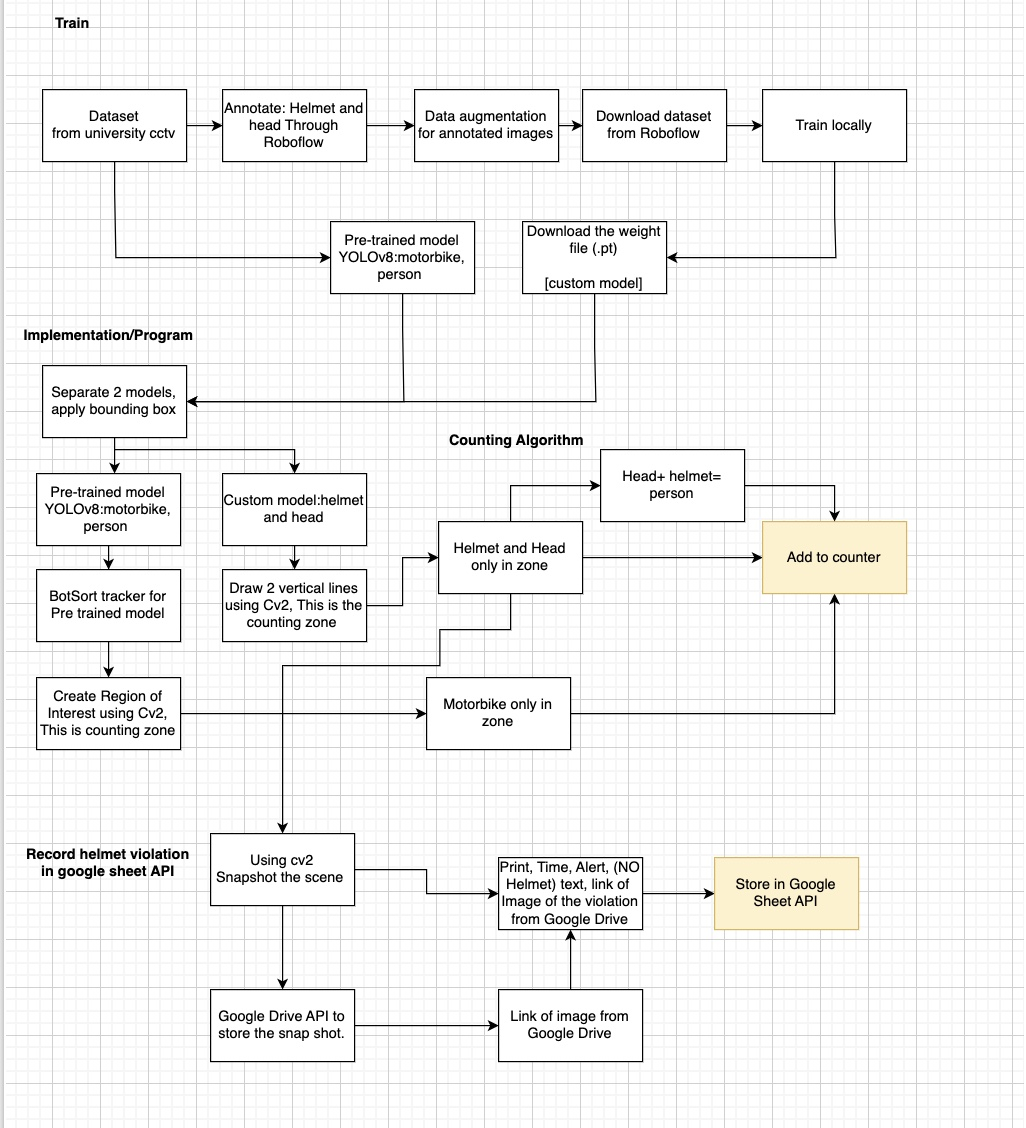
\includegraphics[width=1\textwidth]{flowchart.jpg}
	\vspace{0.5em}
	\noindent\textbf{Figure 3.1} \\
	\caption*{} % Optional: if you want a caption, otherwise keep empty
	
	
\end{figure}

	 The flowchart illustrates the overall workflow of the system. It begins first obtaining the dataset, we obtain them through the cctv footage of the university camera. Specifically spliting the video footages into 3 frames per second using Roboflow. Then annotate each frames splited, the annoated items are helmet and head, then using data augmentations from Roboflow. Then we can downlaod the datasets. Finally, using dataset downloaded we can train locally through data.yaml, the data augmentations details are to be specified in Chapter 3. After the training we will receive the weighted .pt file, the file is the model that will be used in the system in conjunction with the pre-trained model from YOLOv8. The Implementation phase is to apply the models, work with the video stream input. The bounding box and region of interest made from cv2. Using these zone we speparate the counting zone for helmet, head, and another zone to count person and helmet. As for the person we decided to count the head and the helmet to total to person as there are issues about the camera angel limiting the accuracy of the person detection. 
	
	After implementing the program with the model, we use cv2 to take snapshot of the frame as when helmet violation occur. The system links and uses Google API, to store the detection evidence of the scenario. The Google Sheet API will append new rows each time a head detection occur.  The image are visible, and stored by Google Drive API, to check the instances where it happens.
	
\section{Data}
Dataset: videos of riders wearing and not wearing helmets, collected from local sources which is gate six Mahidol University CCTV camera. Videos will then be split in Roboflow which allow custom annotation and training.
\newline
\newline
Annotations: Create two classes. first class containing the bouding box of helmet user only and the second class containing head(which is non-helmet user.)
\newline
Preprocessing: Includes resizing images to 640x640 pixels, normalizing pixel values, and applying augmentations (e.g., rotation, scaling, and brightness adjustments).

\newpage
\section{Custom Model}
\textbf{YOLOv8 Architecture:}
The YOLOv8 architecture was selected for this project due to its state-of-the-art performance in object detection, offering a balance between real-time inference speed and high accuracy. YOLOv8 (You Only Look Once version 8), developed by Ultralytics, is known for its streamlined architecture and improved detection performance over its predecessors (e.g., YOLOv5, YOLOv7), particularly in low-light or occluded environments—conditions often encountered in real-world surveillance footage. Specifically for this project, YOLOv8 is supported by Roboflow, a tool important for training and annotating helmet and head classes easily. Additionally YOLOv8 was easier to set up and supported by developers and communities in a larger scale than other YOLO versions. This will be essentials in debugging and implementing additional tools like trackers. 

Despite the availability of newer object detection models such as YOLO-NAS or YOLOv9, YOLOv8 remains a highly reliable and widely supported choice. In this project, YOLOv8 was used to create a custom-trained model that focuses on five specific object classes: motorcycles, helmets, crosswalks, pedestrians, and lanes. However, the two most critical objects for our safety analysis—helmet and head—were prioritized in both annotation and evaluation.


\begin{center}
	\begin{minipage}{0.45\textwidth}
		\centering
		
\includegraphics[width=\linewidth]{roboflow.png}
		\vspace{0.5em}
		
		\textbf{Figure 3.3.1: Roboflow Image}
	\end{minipage}
	\hfill
	\begin{minipage}{0.45\textwidth}
		\centering
		
\includegraphics[width=\linewidth]{yolo.png}
		\vspace{0.5em}
		
		\textbf{Figure 3.3.2: YOLO Image}
	\end{minipage}
\end{center}

To obtain the custom model for "head", and "helmet" detection we must first upload the datasets into Roboflow website in figure 3.1. Roboflow will allow users to specifically annotate desired classes, which after annotating said datasets, we can download directly from Roboflow the annotated datasets which we can train locally. Training can be done localy or through Google Collab. However due to limitations we used Vistual Studio as a medium to train the datasets from Roboflow. 

\newpage
	
\noindent\textbf{Training Process:} As for our goals the training processes for our custom YOLOv8 model consisted of several key stages, summarized below:

\begin{itemize}
	 \item \textbf{Data Collection:} The dataset was compiled from real CCTV footage recorded on campus at Mahidol University’s Faculty of Engineering. The footage was collected over a span of seven days during the morning rush hour (8:00–10:00 AM), totaling approximately two hours. This time window was chosen to capture peak motorcycle and pedestrian traffic for accurate helmet usage monitoring.  The image below is an example of a snapshot from the dataset, the actually dataset is a video as mention.
\begin{center}
	\includegraphics[width=0.5\textwidth]{Datasets.png}
	
	\vspace{0.5em}
	\textbf{Figure 3.3.3: Dataset Image}
\end{center}
	 
	\item \textbf{Frame extracgtion:} Using the cv2 module from OpenCV, video footage was processed and extracted into still frames. To ensure computational efficiency while retaining sufficient information, frames were sampled at a rate of 3 frames per second (FPS). The extracted images were then uploaded to Roboflow, a computer vision dataset platform, for annotation and augmentation. However for Roboflow they provide a function to slpit the frames within the website and we will be extracting them with Roboflow instead. In the figure below is an example of frame extraction function after uploading the datasets into Roboflow. Extracting the video datasets into frames, means that we can annotate each frames specifically we have three frames across one second. This is to also ensure that we do not have to much datasets, and it also depends on how much the desire classes appears on the videos. For our case there are enough objects across three frames per second to annotate.
	\begin{center}
		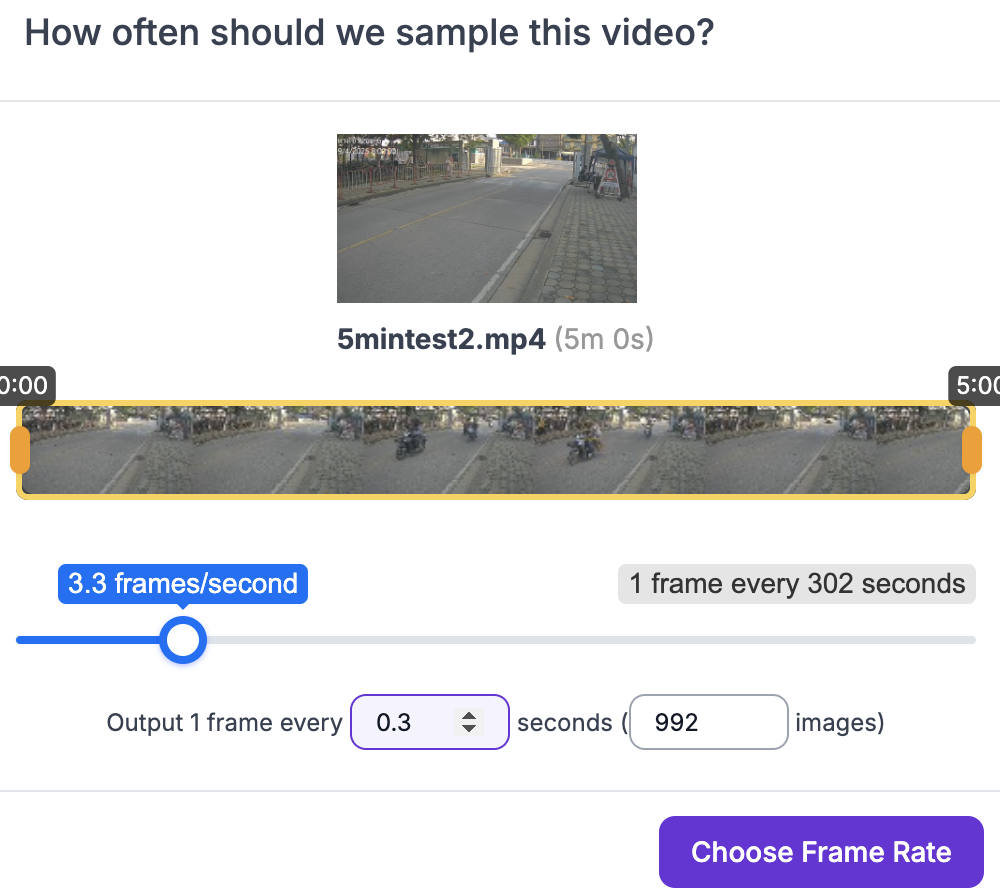
\includegraphics[width=0.5\textwidth]{Frameex.png}
		
		\vspace{0.5em}
		\textbf{Figure 3.3.3: Frame Extraction Image}
	\end{center}
	
	\item\textbf{Annotation:} Within Roboflow, bounding boxes were manually drawn around the target objects—specifically helmets and heads—to create accurate ground truth data for supervised learning. Annotations were carefully reviewed to ensure consistency, especially in challenging cases such as partial occlusions or non-standard helmet designs. The images belows show an example how we draw the bounding boxes for the classes. Drawing the bouding box this way minimizes detection errors and allows the YOLOv8 custom model to focus on the objects more precisely. We encourage to draw the bounding box as close to the objects as possible.
		\begin{center}
		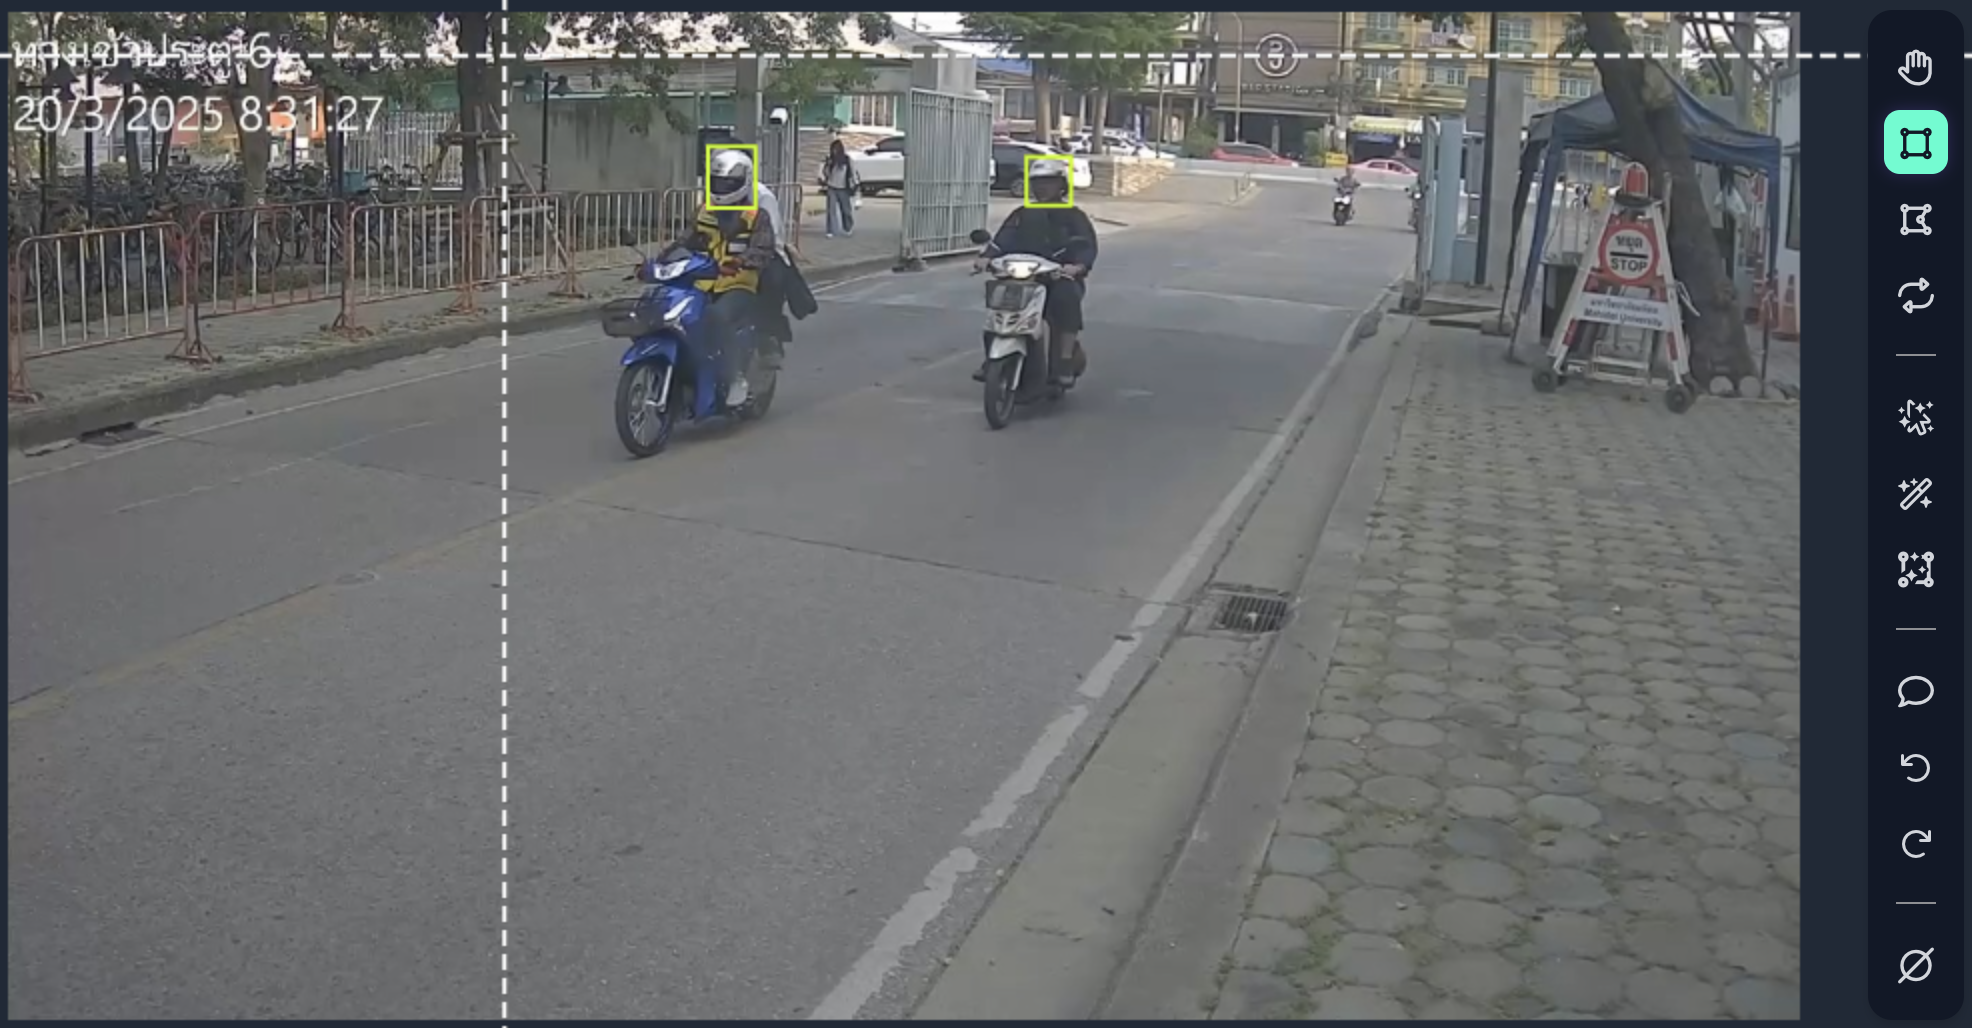
\includegraphics[width=0.8\textwidth]{Anotate.png}
		
		\vspace{0.5em}
		\textbf{Figure 3.3.4: Annotation Image}
	\end{center}
	\newpage
	\item \textbf{Dataset Splitting:}  The annotated dataset was divided into training, validation, and testing sets with a ratio of 70\% training, 20\% validation, and 10]\% testing. This split was chosen to ensure sufficient training samples while preserving a robust validation set to monitor overfitting and a separate test set for unbiased evaluation. Using this data split is widely uses apporach in machine learning as it offers balnce between training, validation, and testing. 70\% of the data use to train allows it to learn patterns from the annotation effectively. It is effieicent and enough for pattern recognition. The 20\% is very important as becuase as this portion is used to check how well the model is learning. Additionally to help tune with the hyperparameters and prevent overfitting. Overfiting occurs when a  model memorizes the training data too well and fails to perform on new, unseen data.  Lastly the 10\% is reserved for testing, for unbaised evaluation of the model. The split ensures thatt the model has enough data to learn, and adjust. This process will occur after completing the annotation process.		
		\begin{center}
		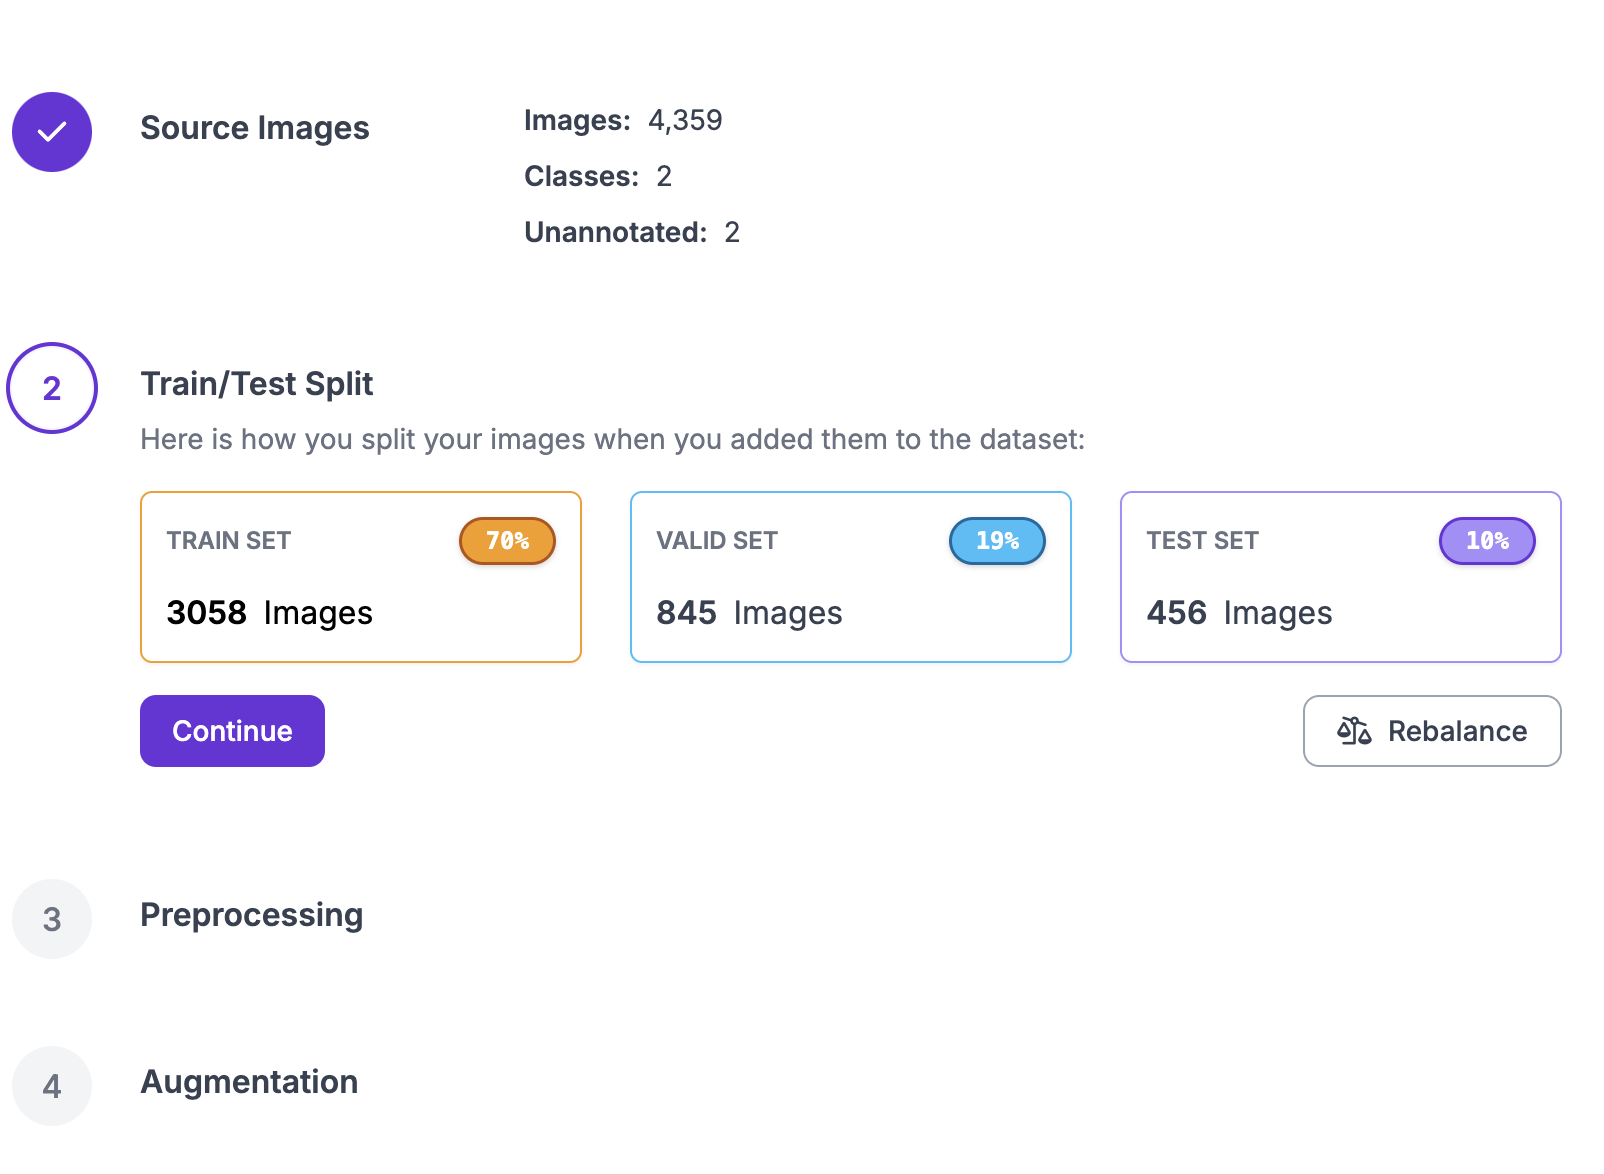
\includegraphics[width=0.8\textwidth]{Split.png}
		
		\vspace{0.5em}
		\textbf{Figure 3.3.5: Spliting Datasets Image}
	\end{center}
	At this step we can also augmentate our data through data augmentation from Roboflow seen in Figure 3.3.5. Data augmentation techniques applied are horizontal flipping, contrast enhancement, and brightness variation were applied to improve the model’s robustness to environmental variations such as lighting conditions or camera angles.
			\begin{center}
		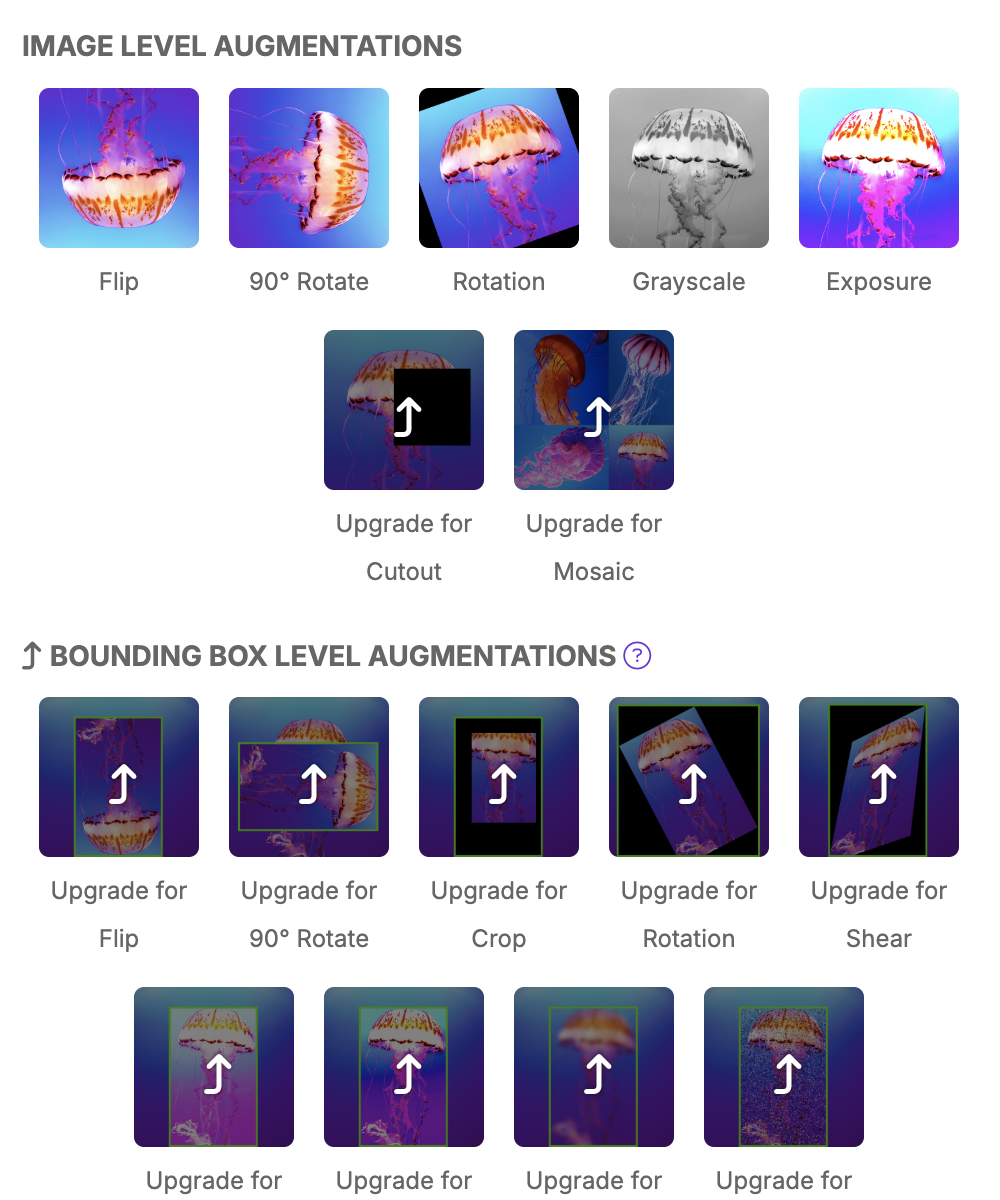
\includegraphics[width=0.8\textwidth]{Augmentation.png}
		
		\vspace{0.5em}
		\textbf{Figure 3.3.6: Augmentation Image}
	\end{center}
	
	\item \textbf{Data Configuration and Training:} Aftering Spliting the data we can download the dataset files from Roboflow. The file will be splited to 70/20/10, train, validate, test. A data.yaml file will have to be  configured to specify class names, dataset paths, and other training parameters. The file is then imported imported into Visual Studio Code (VS Code) for model development and training using the Ultralytics YOLOv8 framework. The images below shows how data.yamlfile is set up.
				\begin{center}
		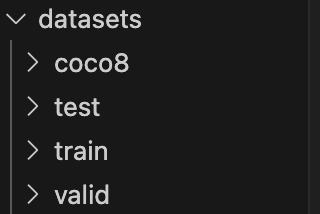
\includegraphics[width=0.8\textwidth]{Files.png}
		
		\vspace{0.5em}
		\textbf{Figure 3.3.7:  Files from downloaded Dataset }
	\end{center}
	 The detailedconfigurations needed used inside data.yaml is located in the Hyperparameter section.
	 Hyperparameters, such as learning rate and non-maximum suppression (NMS) thresholds, were tuned for optimal performance.  After applying the hyparameters, we can start the training through the data.yaml file. After the training has been finish, the wieghted model files will be created in runs/detect. Select the .pt files as a yolo model this will be the model that we will use after all the steps above are complete. For our project be have a total of 4,359 images that are annotated for custom model. The image belows shows the data.yaml content. We will use this to obtain a custom weighted  .pt file.
	 				\begin{center}
	 	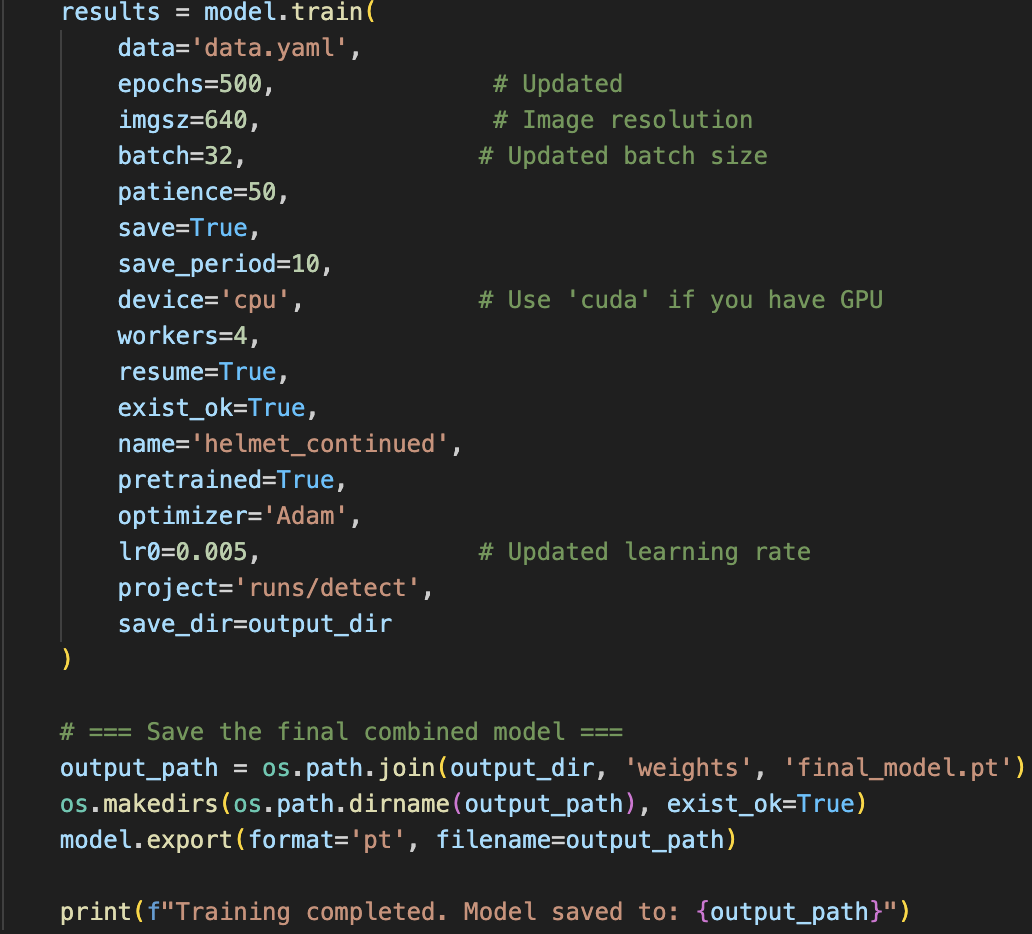
\includegraphics[width=0.8\textwidth]{yaml.png}
	 	
	 	\vspace{0.5em}
	 	\textbf{Figure 3.3.8:  Data.yaml file in VS}
	 \end{center}
\end{itemize}

\section{\textbf{Counting System}}
\subsection{Helmet and Head}

	\noindent\hspace{2.5em}After customizing our YOLOv8 model, we implemented a counting system to track the number of helmets, unhelmeted heads, persons, and motorcycles detected in the video.
	
	
	\noindent\hspace{2.5em}For helmet and head counting, we applied a double-line counting method. This defines a "counting zone" using two vertical lines, and only counts detections whose bounding box centers fall within the zone. To prevent duplicate counting across frames, we used a rolling memory of the last ten frames. If a new detection is within a set distance (e.g., 30 pixels) of a previously counted object of the same type, it is ignored.
	\newline
	This method improves reliability by reducing overcounting and stabilizing results, especially for slow-moving or flickering detections. The final counts are updated in real time and displayed on the video, offering a clear summary of helmet usage and safety compliance.
	\begin{figure}[H] % Optional: [H] requires \usepackage{float}
		\centering
		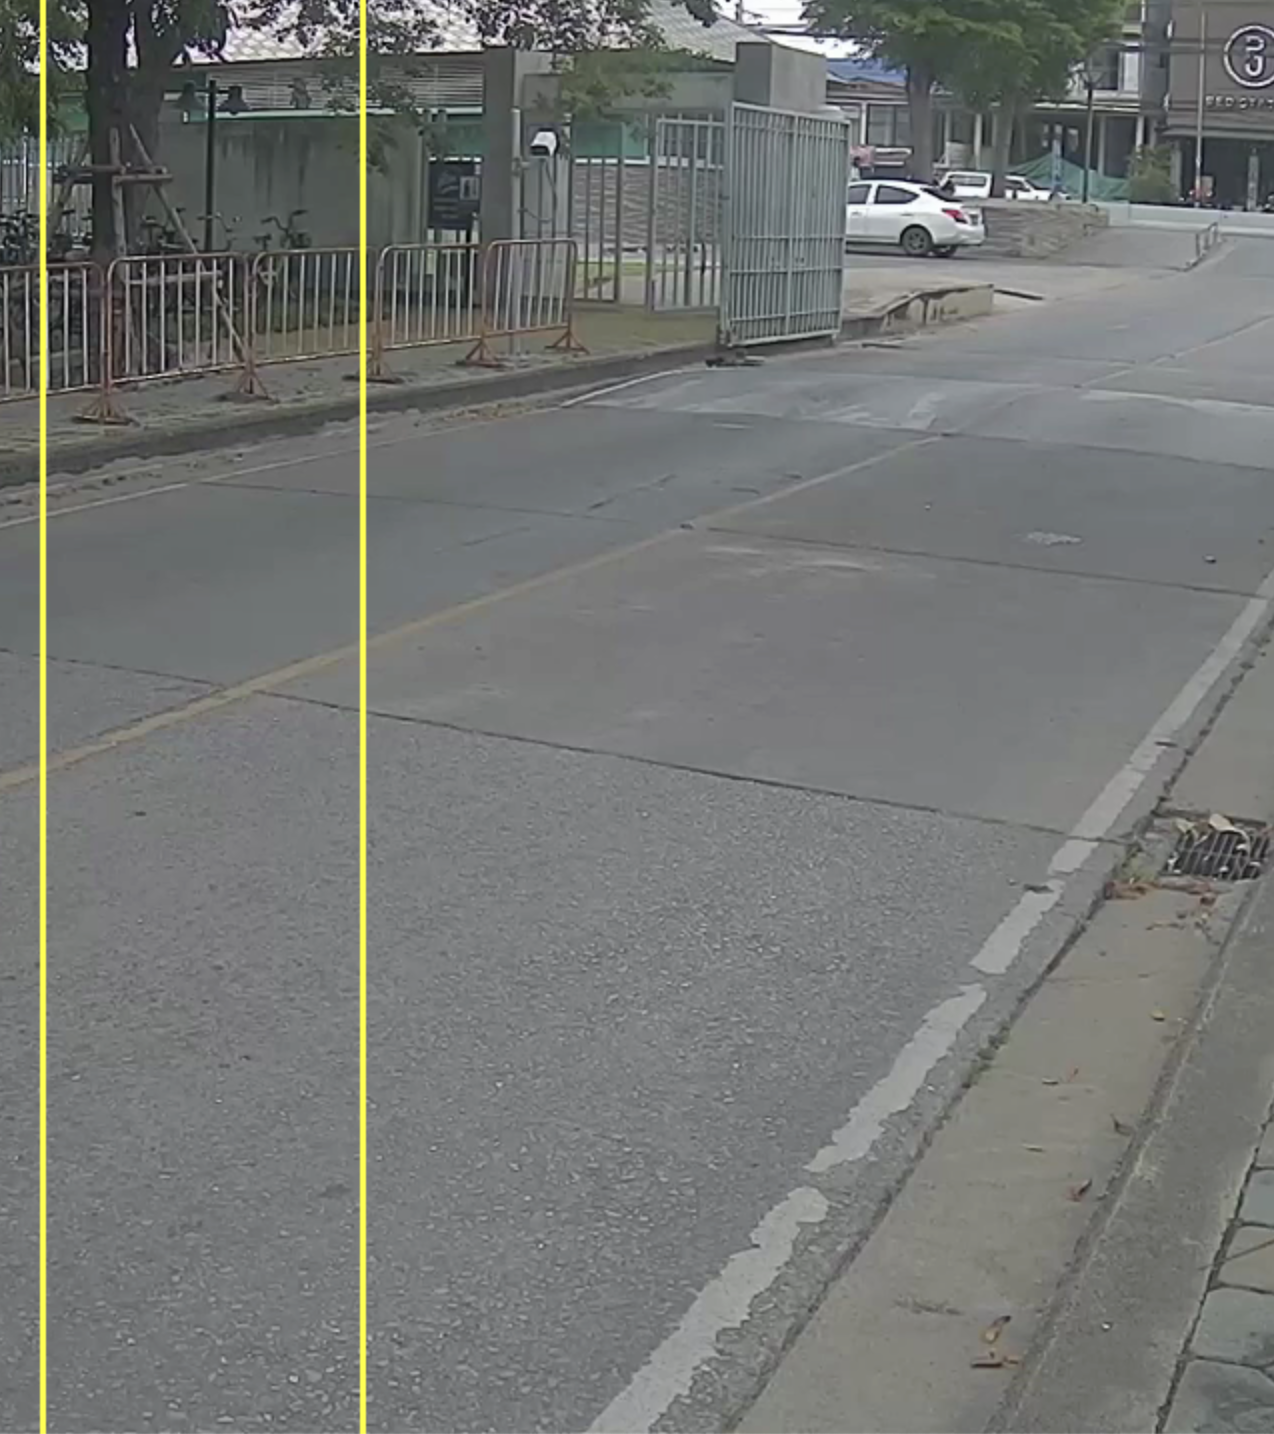
\includegraphics[width=0.5\textwidth]{headhel1.png}
		\vspace{0.5em}
		\caption*{\textbf{Figure 3.2}}
	\end{figure}
	\hfill
	% Right side: Figure 3.3

	\noindent\hspace{2.5em}Figure 3.2 illustrates the designated counting zone used for helmet and head detection. The image shows two vertical yellow lines placed 150 pixels apart, which define the area for double-line counting. When an object passes through both lines in sequence, it is registered as a valid count. This method helps reduce duplicate or false counts caused by temporary detection overlaps or brief tracking loss.
	
	\begin{figure}[H] % Optional: [H] requires \usepackage{float}
		\centering
		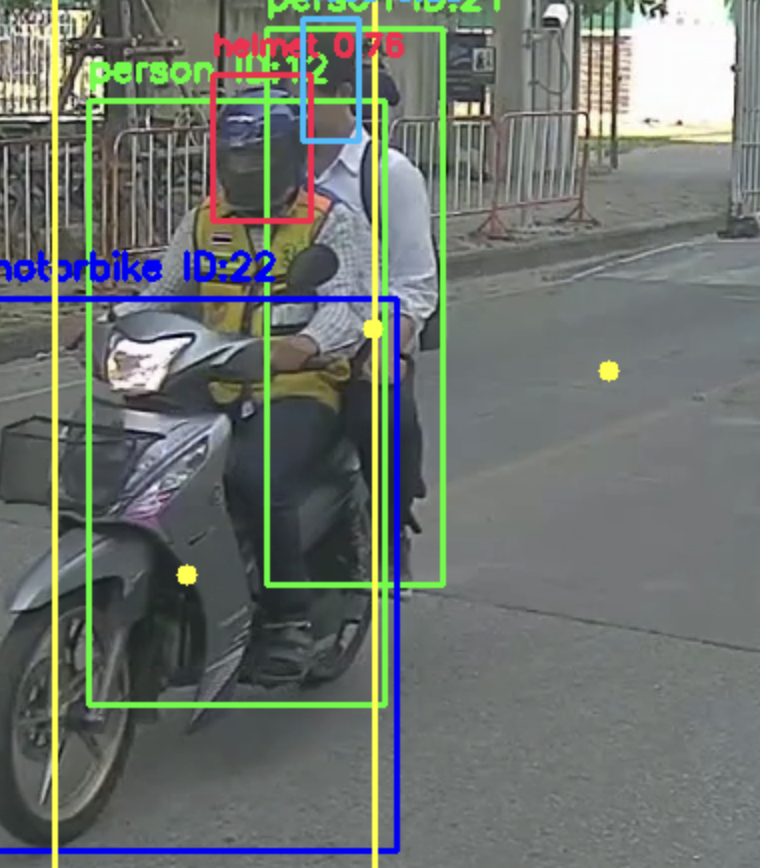
\includegraphics[width=0.5\textwidth]{headhel2.png}
		\vspace{0.5em}
		\caption*{\textbf{Figure 3.3}}
	\end{figure}
	
	\noindent\hspace{2.5em}Figure 3.3 shows an example of the counting system in action when objects, such as a helmet and/or a head, enter the counting zone. As seen in the image, the objects are detected and labeled while passing through the two vertical lines, triggering the counting logic. This illustrates how the system identifies and differentiates helmeted and non-helmeted riders within the defined zone.
	
	\begin{figure}[H] % Optional: [H] requires \usepackage{float}
		\centering
		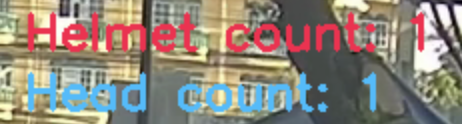
\includegraphics[width=0.5\textwidth]{headhel3.png}
		\vspace{0.5em}
		\caption*{\textbf{Figure 3.4}}
	\end{figure}
	
		\noindent\hspace{2.5em}Figure 3.4 displays the result of the helmet and head counting process, shown at the top-right corner of the screen. These values are updated in real-time after the system detects and counts objects passing through the counting zone. This visual feedback confirms the detection and classification outcome for each rider, distinguishing between helmeted and non-helmeted individuals.
	
	
	
	
\subsection{Person and Motorbike}
\noindent\hspace{2.5em}However as for the Person, and Motorbike detection we can use the Yolov8s.pt model, class 0(person), and class 3(motorbike), as their model are well polished for tracking. For the tracking use Bot-sort tracker, obtain through Roboflow ultralytics/trackers/bot\_sort.py. The tracker will be use to create specific id number for each class that has been detected. Using these id we will create center point of each classes which will be important in the counting method.


\noindent\hspace{2.5em}For the counting method, we can create a region of interest, through using open CV. From there we create a condition, to store the track id with track history. track\_history = {}   function will store the position cx, cy of the tracked object. We will use this value to identify its current and previous position to ensure that when object inside the Region of Interest, position compare is is greater than the current position objected will not be used to count, while if the current position of the tracked id compared to stored id is less than it, it can be counted inside the ROI. This is to ensure that the person, and motorbike can be counted by by what it can be tracked. The detection should look similiar to figure1.

\begin{center}
	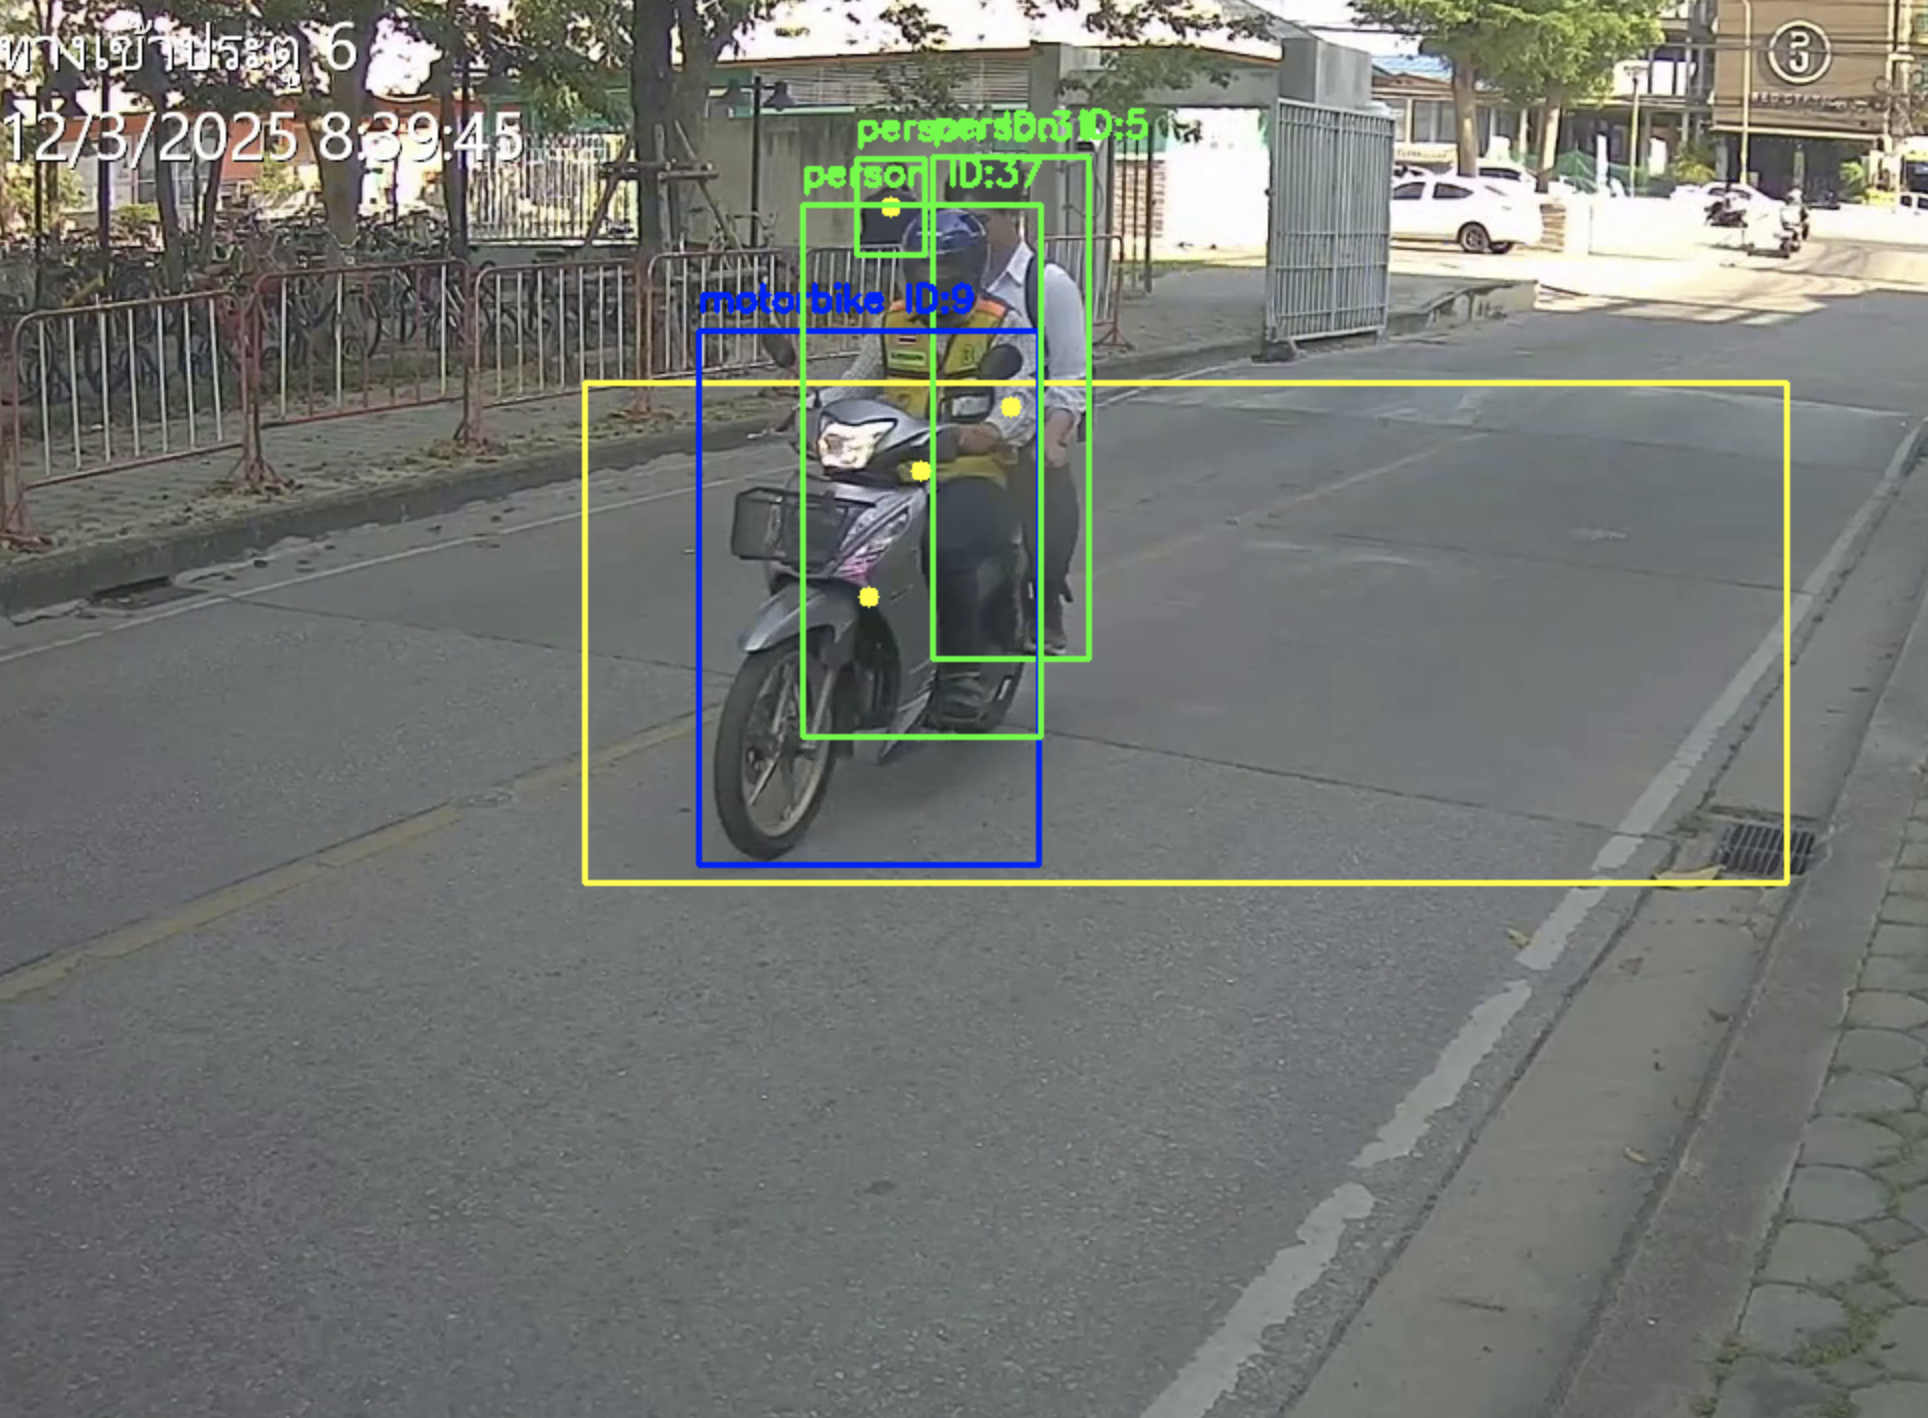
\includegraphics[width=0.5\textwidth]{fig1.png}
	
	\vspace{0.5em}
	\textbf{Figure 3.5}
\end{center}


\subsection{Output Generation}
\noindent\hspace{2.5em}The output generation phase transforms the detection and counting results into a visual and interpretable format. For each processed video frame, the system overlays bounding boxes and labels indicating the object class (helmet, head, person, or motorcycle), along with live counts displayed on the top-left corner using OpenCV. These real-time visual indicators allow users to monitor helmet usage compliance at a glance. Additionally, the system can produce an annotated video file as output, which includes all detections and updated counts across the entire duration. This output is valuable for both immediate observation and later review or reporting, providing a clear and documented summary of safety compliance in the monitored area. The images below shows the output of the system which after we run the program, will show live dection of the video input, and the save video file after the program completed the detection, we save it as a way to easier analyse and observe the detection through video playback, as analysing it live while running maybe not be as efficient.
\begin{center}
	\begin{minipage}{0.45\textwidth}
		\centering
		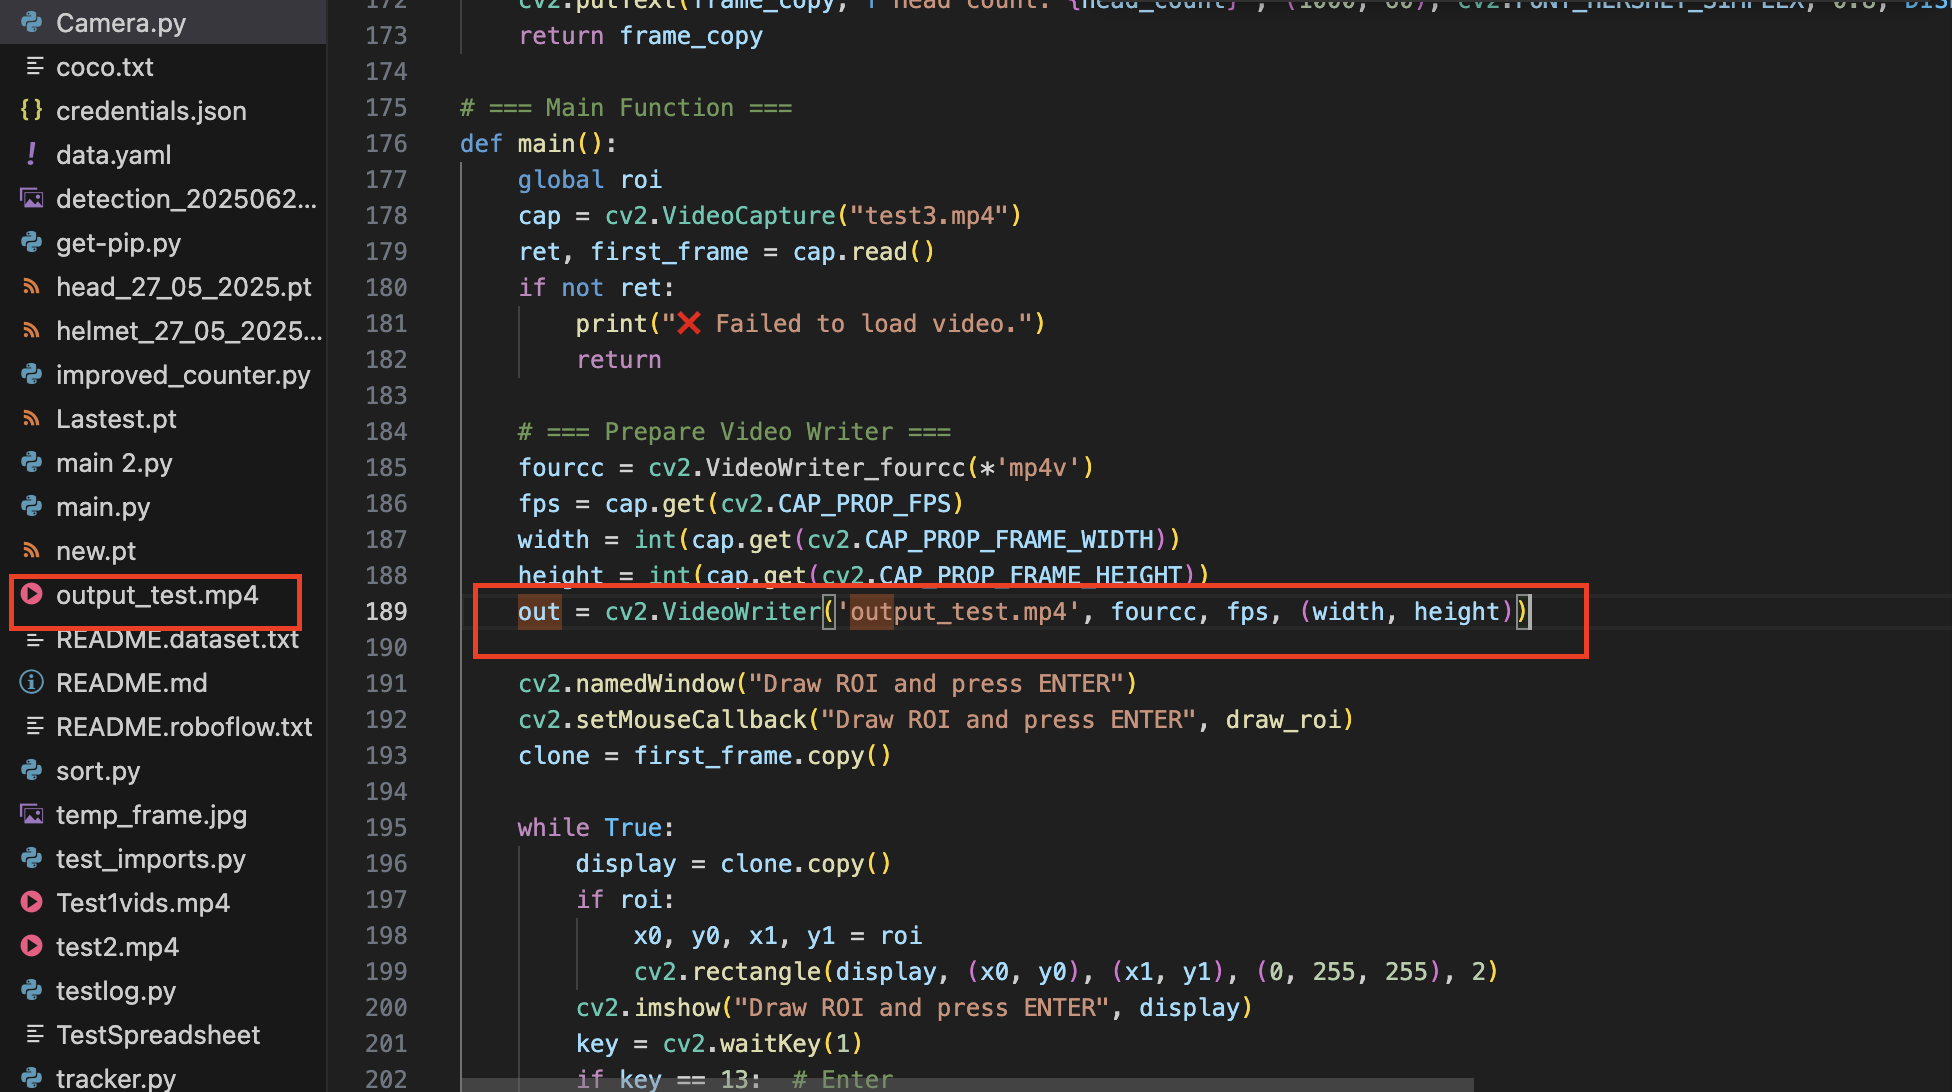
\includegraphics[width=\linewidth]{out.png}
		\vspace{0.7em}
		
		\textbf{Figure 3.4.1: Saved output Video}
	\end{minipage}
	\hfill
	\begin{minipage}{0.45\textwidth}
		\centering
		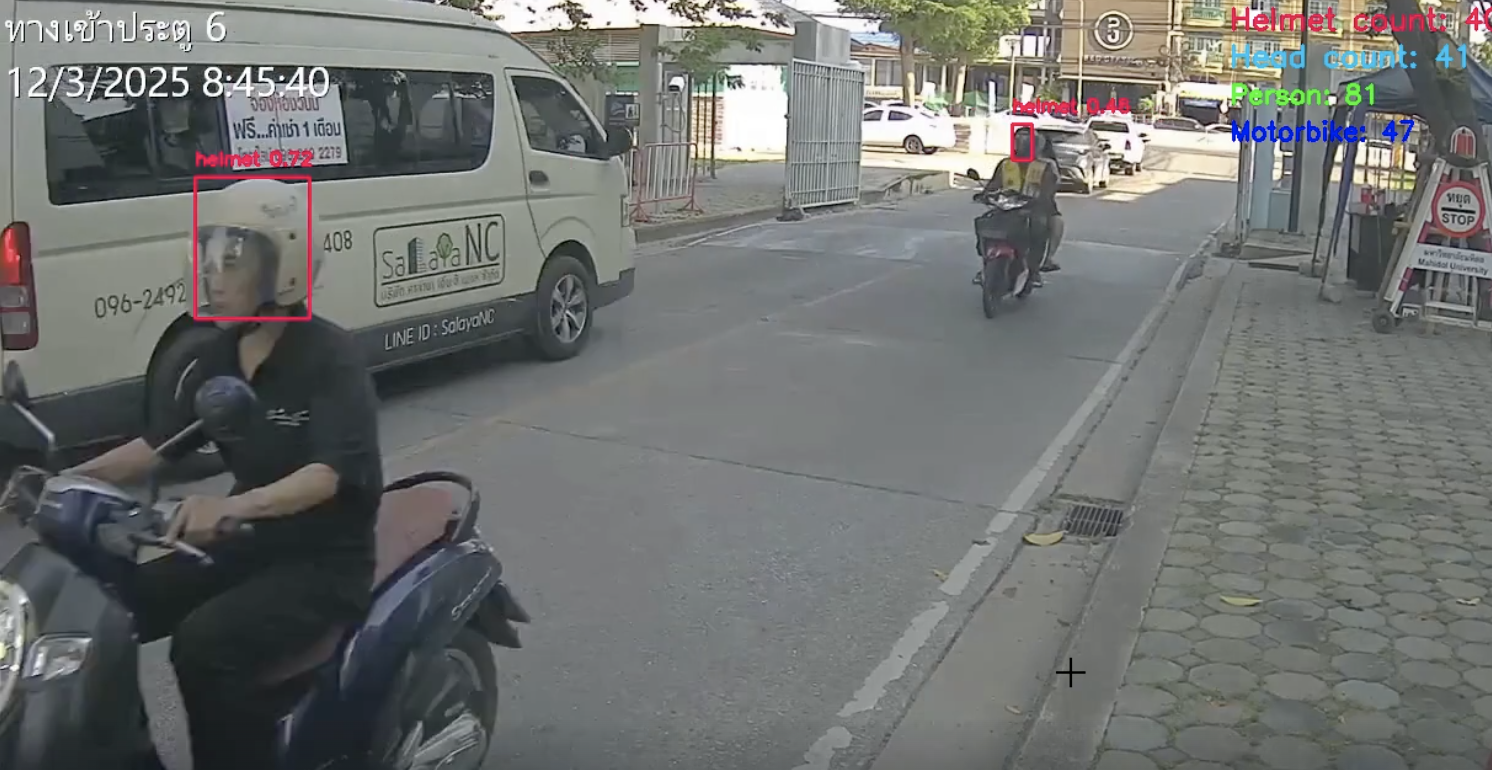
\includegraphics[width=\linewidth]{live.png}
		\vspace{0.5em}
		
		\textbf{Figure 3.4.2: Live Output Generation}
	\end{minipage}
\end{center}


\subsection{Storing Output in Google Sheet API}
\noindent\hspace{2.5em}After the output has been generated, we store the detection into a log using Google API from the video steam. The Google API integration is used for logging and evidence storage for helmet violation cases. Firstly as mention the two model, YOLOv8 pre-trained model, and custom model for head/helmet detection. How the system is works is, when a head is detected within the zone. The frames will be stored, using cv2 to snap-shot the specific frame of head detection. We log the detections events to Google Sheet, it records, the timestamp, head detection, alert, and link to Google Drive file to the captured image.


\noindent\hspace{2.5em}The credentials.json file can be obtained through Google API, the system will connect to pre-defined Google Sheet as we name them(Data log) and appneds the new rows with each detection events that occurs, the image are uploaded to Google Drive using the Drive API, and public access links are generated per log. This implementation allows users to store datas of the detection, this is to allow scalable and automated solution for monitoring helmet violations. The result is as seen in the figure below.

\begin{center}
	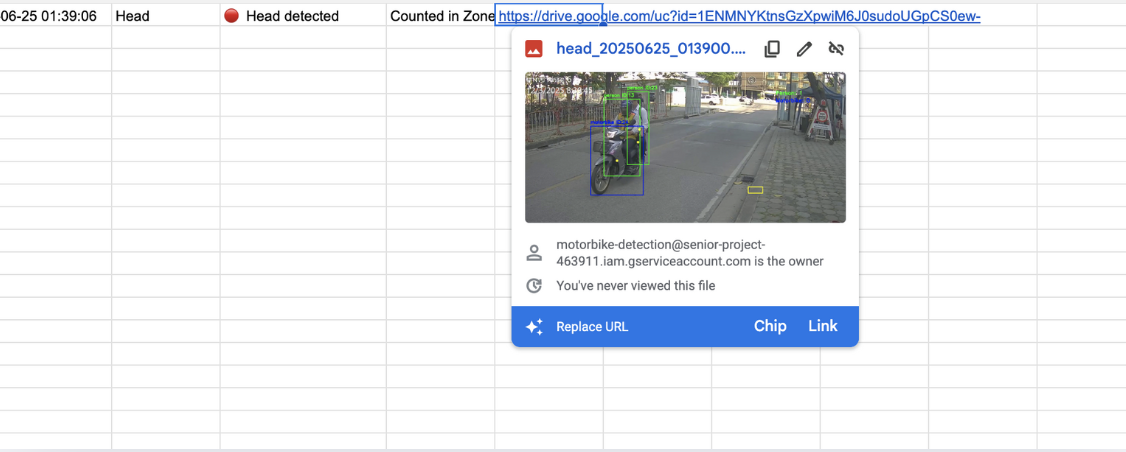
\includegraphics[width=1\textwidth]{api.png}
	
	\vspace{0.5em}
	\textbf{Figure 3.6}
\end{center}

\section{Tools and Frameworks}
\begin{itemize}
	\item \textbf{YOLOv8 Framework}: For object detection.
	\item \textbf{Libraries}: Python libraries such as ultralytics, opencv-python, numpy, collections.
	\item \textbf{Annotation Tools}: Roboflow.
	
\end{itemize}


\section{Hyperparameter Configurations}
During the training process, serveral key herparameters were carefufully selected to balace the performce, the model accuracy and accordingly to our local computation resrouces.

\textbf{Epochs} = 500, this is to ensure suffieicent exposeure to the training datasets. It will allow the model to learn patterns, and improve generalization overtime. However we can stop the early depending on our resources and depending on overfitting.

\textbf{Image Size} imgsz = 640 (image resolution) 640x640 pixel is most commonly use parameter. This will also help decrease the traning time. However for smaller objects like head and helmet detection. Training them on 640x640 is enough, however in some circumstances when training very far, helmet and head that are annotated are risk to losing fine-grained details. This is important as it is very essential for detecting small overlapping objects. For our case we annotate them after they pass the bumper, we have checked that at this area before hand that when resolution was 640x640, it was not too grainy for traing. The image belows shows the annotated image that was resized to 640x640 for training. 


\begin{center}
	\begin{minipage}{0.45\textwidth}
		\centering
		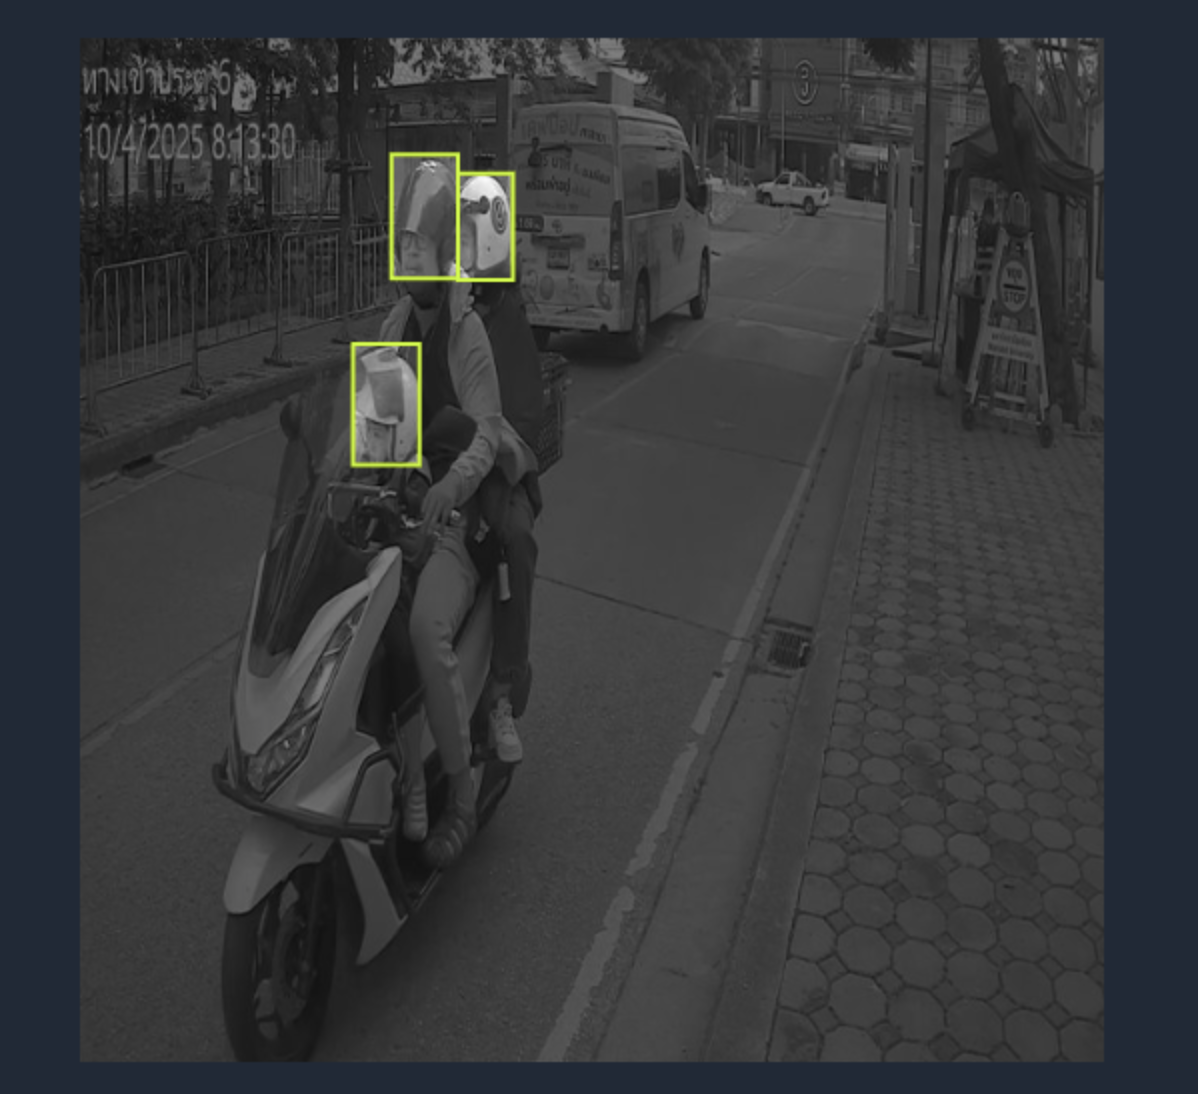
\includegraphics[width=\linewidth]{ano1.png}
		\vspace{0.7em}
		
		\textbf{Figure 3.6.1: Resized Image }
	\end{minipage}
	\hfill
	\begin{minipage}{0.45\textwidth}
		\centering
		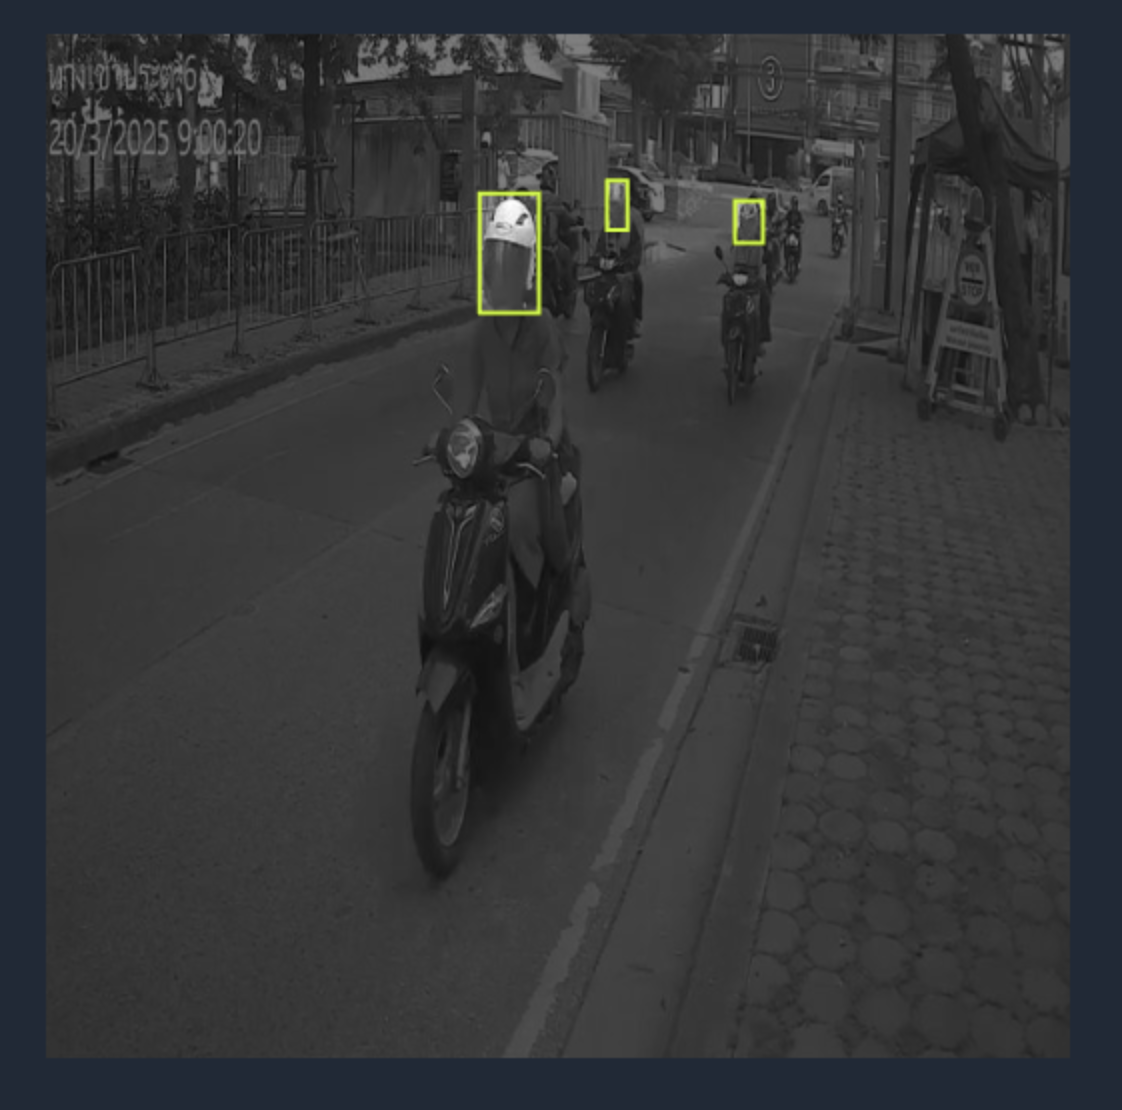
\includegraphics[width=\linewidth]{ano2.png}
		\vspace{0.5em}
		
		\textbf{Figure 3.6.2: Resized Image }
	\end{minipage}
\end{center}




\textbf{Batch Size} =32, this is due to primarily contrained by the GPU, as larger batches can lead larger samples, and faster convergency. Nonetheless, batch size 32istill alowws for reasonable effieicnt traning and consistent model updates. This value can be changed depending on the GPU memory. While a larger batch size could have potentially accelerated training and stabilized gradient updates, our hardware limitations required a compromise at 32 images per batch.

\textbf{Learning Rate} = 0.005. Setting it to this value helps to cacilitate steady learning without causing instability. If it was too high, it could result in model to overshoot the optimal solution during traning. This value is also recommended by YOLOv8.



\section{Performace Evaluation}

\noindent\hspace{2.5em}The trained YOLOv8 model was evaluated using:
mAP: To quantify detection accuracy.
Confusion matrix: To identify true positives, false positives, and negatives.
The purpose of the performance evaluation is to help our team, look at the development of the different models. The benefits of finding the best model is to use them for the best accuracy for the counting systems.

\begin{center}
	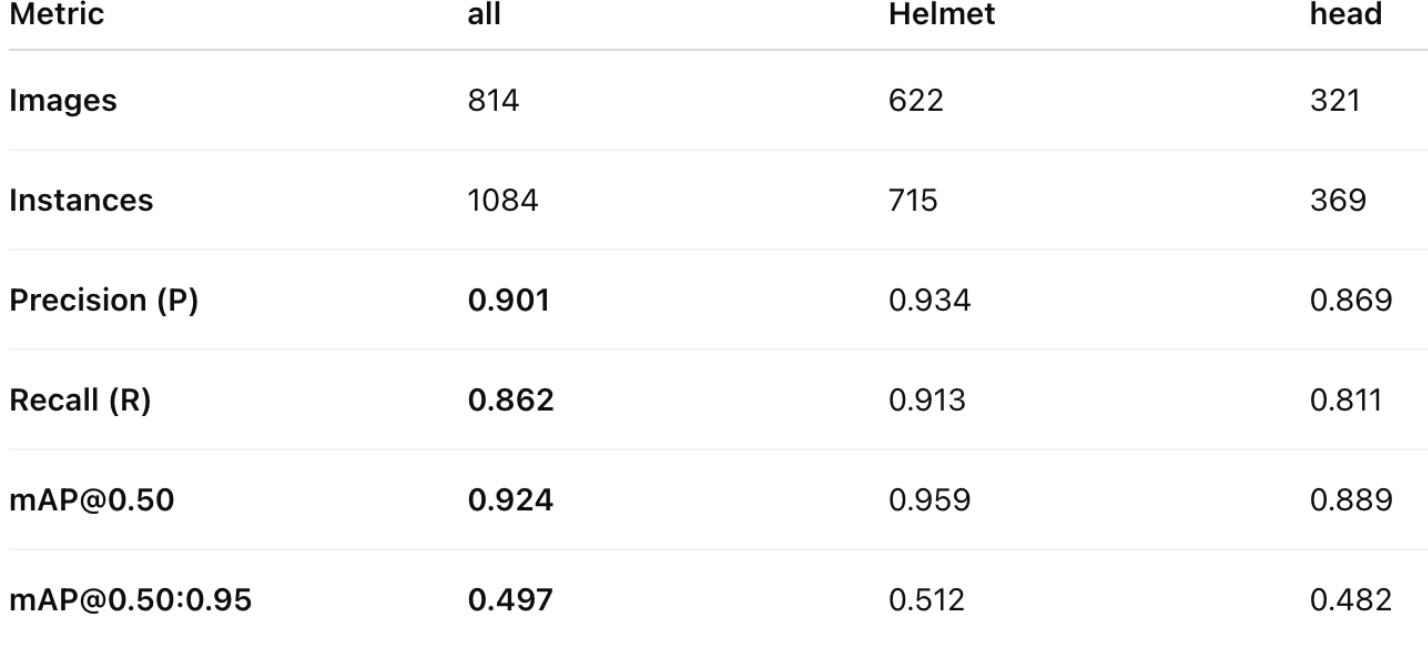
\includegraphics[width=1\textwidth]{performance.eva.png}
	
	\vspace{0.5em}
	\textbf{Figure 3.7}
\end{center}

\noindent\hspace{2.5em}The evaluation results in figure 3.7 demonstrate that the best custom YOLOv8 model performs strongly in detecting both helmet and heads(non-helmet), with particularly high accuracy in helmet detection. Overall, the model achieved a precision of 0.901 and recall of 0.862 across all classes, indicating reliable and consistent predictions. For the helemt class specifically, the model attained satisfying performance with a precision of 0.934, recall of 0.913, and a high mAP@0.50 of 0.959. This suggests that the model can effectively identify helmets with minimal false positives and false negatives. In comparison, the head class yielded slightly lower results, with a precision of 0.869, recall of 0.811, and mAP@0.50 of 0.889, reflecting more variation or complexity in detecting uncovered heads. The overall mAP@0.50:0.95 score of 0.497, while moderate, still indicates acceptable performance under stricter localization conditions. These results affirm the model’s suitability for real-time helmet usage monitoring, particularly in scenarios where accurate helmet detection is critical.

\begin{center}
	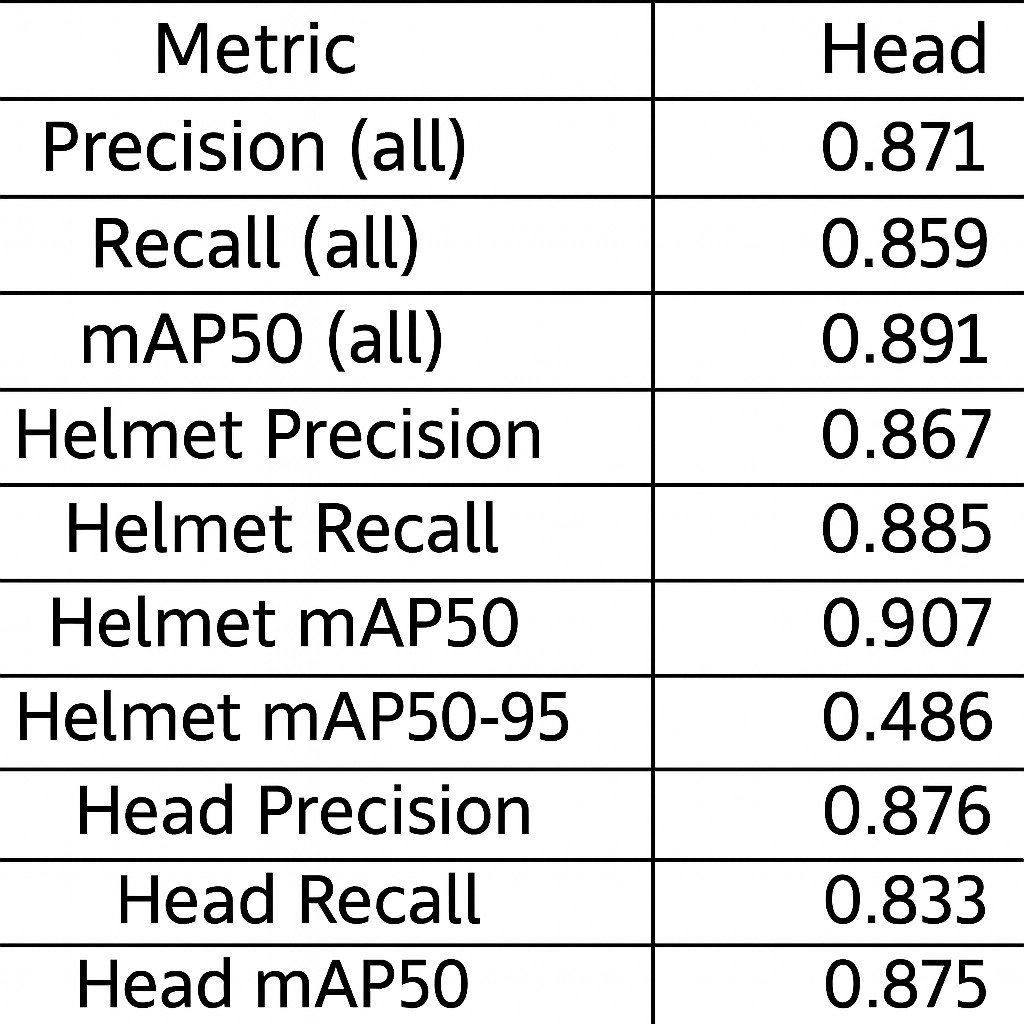
\includegraphics[width=0.5\textwidth]{performance.eva2.png}
	
	\vspace{0.5em}
	\textbf{Figure 3.8}
\end{center}
\noindent\hspace{2.5em}Figure 3.8 shows the previous model performace evaluation, which is call Head\_model. In comparing the performance of the updated helmet and head detection model, which is figure 3.7, to the previous version, several improvements are evident. 

\noindent\hspace{2.5em}The current model achieves an overall precision of 0.901 and recall of 0.862, both higher than the previous model’s precision of 0.871 and recall of 0.859, suggesting better accuracy and detection coverage. Helmet detection has particularly improved, with the current model reaching a helmet precision of 0.934, recall of 0.913, and mAP@0.50 of 0.959, outperforming the previous model’s respective values of 0.867, 0.885, and 0.907. Head detection has also seen slight gains, with the current model achieving 0.869 precision, 0.811 recall, and 0.889 mAP@0.50, compared to 0.876, 0.833, and 0.875 in the earlier version. Additionally, the current model maintains a solid mAP@0.50:0.95 of 0.497 overall, indicating better localization performance under stricter IoU thresholds. These enhancements reflect a more robust and reliable detection system, making the current model better suited for real-world deployment in helmet compliance monitoring scenarios.
